% Options for packages loaded elsewhere
\PassOptionsToPackage{unicode}{hyperref}
\PassOptionsToPackage{hyphens}{url}
\PassOptionsToPackage{dvipsnames,svgnames,x11names}{xcolor}
%
\documentclass[
  abstract]{article}

\usepackage{amsmath,amssymb}
\usepackage{iftex}
\ifPDFTeX
  \usepackage[T1]{fontenc}
  \usepackage[utf8]{inputenc}
  \usepackage{textcomp} % provide euro and other symbols
\else % if luatex or xetex
  \usepackage{unicode-math}
  \defaultfontfeatures{Scale=MatchLowercase}
  \defaultfontfeatures[\rmfamily]{Ligatures=TeX,Scale=1}
\fi
\usepackage{lmodern}
\ifPDFTeX\else  
    % xetex/luatex font selection
\fi
% Use upquote if available, for straight quotes in verbatim environments
\IfFileExists{upquote.sty}{\usepackage{upquote}}{}
\IfFileExists{microtype.sty}{% use microtype if available
  \usepackage[]{microtype}
  \UseMicrotypeSet[protrusion]{basicmath} % disable protrusion for tt fonts
}{}
\usepackage{xcolor}
\usepackage[margin=1.1in,letterpaper]{geometry}
\setlength{\emergencystretch}{3em} % prevent overfull lines
\setcounter{secnumdepth}{5}
% Make \paragraph and \subparagraph free-standing
\ifx\paragraph\undefined\else
  \let\oldparagraph\paragraph
  \renewcommand{\paragraph}[1]{\oldparagraph{#1}\mbox{}}
\fi
\ifx\subparagraph\undefined\else
  \let\oldsubparagraph\subparagraph
  \renewcommand{\subparagraph}[1]{\oldsubparagraph{#1}\mbox{}}
\fi


\providecommand{\tightlist}{%
  \setlength{\itemsep}{0pt}\setlength{\parskip}{0pt}}\usepackage{longtable,booktabs,array}
\usepackage{calc} % for calculating minipage widths
% Correct order of tables after \paragraph or \subparagraph
\usepackage{etoolbox}
\makeatletter
\patchcmd\longtable{\par}{\if@noskipsec\mbox{}\fi\par}{}{}
\makeatother
% Allow footnotes in longtable head/foot
\IfFileExists{footnotehyper.sty}{\usepackage{footnotehyper}}{\usepackage{footnote}}
\makesavenoteenv{longtable}
\usepackage{graphicx}
\makeatletter
\def\maxwidth{\ifdim\Gin@nat@width>\linewidth\linewidth\else\Gin@nat@width\fi}
\def\maxheight{\ifdim\Gin@nat@height>\textheight\textheight\else\Gin@nat@height\fi}
\makeatother
% Scale images if necessary, so that they will not overflow the page
% margins by default, and it is still possible to overwrite the defaults
% using explicit options in \includegraphics[width, height, ...]{}
\setkeys{Gin}{width=\maxwidth,height=\maxheight,keepaspectratio}
% Set default figure placement to htbp
\makeatletter
\def\fps@figure{htbp}
\makeatother

\makeatletter
\@ifpackageloaded{caption}{}{\usepackage{caption}}
\AtBeginDocument{%
\ifdefined\contentsname
  \renewcommand*\contentsname{Table of contents}
\else
  \newcommand\contentsname{Table of contents}
\fi
\ifdefined\listfigurename
  \renewcommand*\listfigurename{List of Figures}
\else
  \newcommand\listfigurename{List of Figures}
\fi
\ifdefined\listtablename
  \renewcommand*\listtablename{List of Tables}
\else
  \newcommand\listtablename{List of Tables}
\fi
\ifdefined\figurename
  \renewcommand*\figurename{Figure}
\else
  \newcommand\figurename{Figure}
\fi
\ifdefined\tablename
  \renewcommand*\tablename{Table}
\else
  \newcommand\tablename{Table}
\fi
}
\@ifpackageloaded{float}{}{\usepackage{float}}
\floatstyle{ruled}
\@ifundefined{c@chapter}{\newfloat{codelisting}{h}{lop}}{\newfloat{codelisting}{h}{lop}[chapter]}
\floatname{codelisting}{Listing}
\newcommand*\listoflistings{\listof{codelisting}{List of Listings}}
\makeatother
\makeatletter
\makeatother
\makeatletter
\@ifpackageloaded{caption}{}{\usepackage{caption}}
\@ifpackageloaded{subcaption}{}{\usepackage{subcaption}}
\makeatother
\ifLuaTeX
  \usepackage{selnolig}  % disable illegal ligatures
\fi
\usepackage[sorting=none, style=numeric-comp]{biblatex}
\addbibresource{/Users/mt/workspace/Writing/library.bib}
\usepackage{bookmark}

\IfFileExists{xurl.sty}{\usepackage{xurl}}{} % add URL line breaks if available
\urlstyle{same} % disable monospaced font for URLs
\hypersetup{
  pdftitle={Foundational claims of group polarization are plausibly false, with lessons for the empirical study of psychological dynamics},
  colorlinks=true,
  linkcolor={blue},
  filecolor={Maroon},
  citecolor={Blue},
  urlcolor={Blue},
  pdfcreator={LaTeX via pandoc}}

\usepackage{authblk}
\usepackage{etoolbox}
\makeatletter
\title{Foundational claims of group polarization are plausibly false,
with lessons for the empirical study of psychological dynamics}
\makeatother
\author[1,*]{{Matthew A.~Turner}}
\affil[1]{\small Division of Social Sciences, Stanford Doerr School of Sustainability, Stanford University}

\author[2,3]{{Paul E.~Smaldino}}
\affil[2]{\small Cognitive and Information Sciences, University of California, Merced}
\affil[3]{\small Santa Fe Institute} 
% \vspace{2em}
\affil[*]{\small Correspondence: \href{mailto:maturner@stanford.edu}{maturner@stanford.edu}}

\date{}
\begin{document}
\maketitle
\begin{abstract}
\noindent \emph{Group polarization} is the name for a form of consensus
where members of a like-minded group become, on average, more extreme in
their opinions after discussing a topic. Group polarization is important
because it may drive political polarization if moderate partisans become
more extreme. Theoretically, group polarization is celebrated as a
regular, reliable outcome of a certain experimental design based on
dozens of published studies that purportedly demonstrate the phenomena.
However, in this paper we show that 55 of 60 published observations of
purported group polarization, from ten foundational studies, are equally
well-explained by a simple consensus model where group opinion variance
decreases, but extremity does not increase. We use a novel computational
meta-analysis framework designed to identify plausible pre- and
post-discussion opinion distributions that are consistent with simple
consensus, but appear to be group polarization when measured on ordinal,
Likert-style scales. This occurs due to ceiling effects induced by
ordinal measurements. At best this shows that a selection of
foundational research in social psychology must be discarded. At worst
this is the tip of the iceberg, and many similar social psychological
findings within and without the group polarization tradition will
similarly be shown to be unreliable.
\end{abstract}

\renewcommand*\contentsname{Table of contents}
{
\hypersetup{linkcolor=}
\setcounter{tocdepth}{3}
\tableofcontents
}
\begin{quote}
In our introductory social psychology course, 
we have for many years used the [group polarization experimental paradigm] as
a laboratory exercise. The exercise works beautifully, but one must be
careful to forewarn a class that [group polarization] does not occur with every 
group\ldots and that the effect is not large. 
\par\raggedleft(Brown, 1986, p.\cite[p. 205]{Brown1986})
\end{quote}

\begin{quote}
One of the most robust findings in social psychology is that of attitude polarization 
following discussion with like-minded others.
\par\raggedleft(Cooper et al, 2001, p. 267 \cite[p. 267]{Cooper2001})
\end{quote}

\section{Introduction}\label{introduction}

Unchecked social and political polarization undermines cooperation and
political efficacy \autocite{Mason2018UncivilAgreementBook,Klein2020}.
\emph{Group polarization} is the name for a group-level process that
leads to greater opinion extremity in a group as the group deliberates
some topic (e.g., ``Do you approve, disapprove, or neither approve nor
disapprove of the current administration's policies?''). Extremity only
increases, though, assuming that the mean opinion of the group is
initially biased towards one extreme or the other
\autocite{Brown1986,Brown2020}. Group polarization is important to
understand rigorously, therefore, since if groups become increasingly
extreme over time, while group opinions are consolidated, this would
exacerbate political polarization between political opposition groups,
which is already undermines the ability of partisans in democratic
governments to work together. Dozens of studies and meta-analyses over
decades have apparently established the empirical reality of group
polarization
\autocite{Moscovici1969,Myers1970,Isenberg1986,Sunstein2009,Sunstein2019}
\autocite[Ch. 5]{Brown2000}. We believe group polarization should occur
in certain contexts since more extreme group members are likely also to
be more stubborn \autocite{Guazzini2015,Lewandowsky2019}, which should
pull consensus to extremes \autocite{Turner2020}. However, many or most
of the evidence for group polarization relies on experimental designs
that use ordinal measurements that are then analyzed as if they were
continuous. Unfortunately, this procedure is unfortunately known to
induce false positives if it is not properly accounted for
\autocite{Liddell2018}.

Experimetnal designs in group polarization studies share a certain
experimental boilerplate (Figure 1 --- NEED TO INCLUDE) with the goal of
testing the group polarization hypothesis that a group of like-minded
people will develop more extreme opinions on some salient topic over the
course of discussing some topic. Group polarization experiments are thus
initialized by forming like-minded groups of people and surveying their
initial opinions on some topic. In some cases these initial opinions are
used for assigning participants to like-minded groups, but other methods
have been used, such as geographic location for producing, on average,
like-minded groups \autocite{Schkade2010}. Participants then discuss the
topic in their groups. After discussion, participant opinions are again
measured. Several studies we analyze here determined group polarization
occurred (i.e., defined a positive detection) only as a non-zero
difference in mean opinion, with no other statistical testing. Some
others performed null-hypothesis \(t\)-tests to test whether there was
enough evidence to reject the null-hypothesis that \emph{simple
consensus} occurredand not group polarization. In our meta-analysis
simulations, we measure simulated group polarization effect size in
terms of Cohen's \(d\), which is an abstraction beyond these two
practices from the group polarization literature that can also be used
to compare model fits between metric models that treat group
polarization measurements as continuous although they are ordinal, and
more appropriate statistical models that account for data ordinality.

In this paper, we perform a meta-analysis of sixty detections of group
polarization from ten published research articles and show that
fifty-five of the sixty cannot be reliably identified as group
polarization. We show that these 55 are plausibly false detections
because they are equally well-explained by a \emph{simple consensus}
model, where the mean group opinion is unchanged by group discussion but
opinion variance decreases. Theoretically, consensus occurs when
sufficiently like-minded individuals influence, which decreases group
opinion variance \autocite{DeGroot1974,Turner2018}. Group polarization,
then, is consensus plus an overall increase in group opinion extremity,
i.e., an increase in mean group opinion after discussion. We use a novel
approach, described herein, that enabled us to identify continuous pre-
and post-discussion simple consensus opinion distributions that result
in data that appear to be group-polarized when opinions are drawn from
these distributions and measured with an ordinal scale. This approach
could be adapted for similar social psychological studies that used
ordinal measures to determine whether change occurred in distributions
of continuous psychological variables such as opinions and beliefs. For
social psychology and group polarization, this means that an accepted,
heretofore unquestioned, empirical fact must be re-evaluated.
Experimental designs in the field must be updated if we are to
rigorously understand whether and when group polarization occurs.

\subsection{Studies included in this
meta-analysis}\label{studies-included-in-this-meta-analysis}

We chose the ten studies guided by a desire to identify foundational
studies that contribute to the general consensus in social psychology
that group polarization reliably occurs across experimental
settings---one author of one of the ten journal articles is a law
professor who has written two trade books on group polarization to argue
that group polarization occurs in real-world settings in addition to the
laboratory, with political and other practical importance
\autocite{Sunstein2009,Sunstein2019}. We chose studies that either had a
significant influence on the study of group polarization and social
psychology, in terms of a high citation count or adaptation in
popularized trade books, or were designed to support one of four
prominent theoretical explanations of group polarization. The studies
must also have used an ordinal scale for measuring participant opinions
(all but a handful of exceptions use ordinal measurements to measure
group polarization; e.g.~blackjack bets
\autocite{Blascovich1973,Blascovich1976} and mock jury monetary damages
\autocite{Schkade2000}). We included at least one study that supported
or was motivated by one of four established theoretical explanations
(introduced below) of group polarization to show all have at least some
supporting evidence that must be discarded. We also included two studies
that lack a clear theoretical motivation. For the sake of orienting the
reader to the group polarization literature and as a useful organizing
feature for our analysis, we now introduce the theories that motivate
eight of the ten studies. To further orient the reader, we then provide
details of the experimental designs used to produce the 60 published
positive detections of group polarization across 10 research articles
that we scrutinize here. Group polarization experimental designs are
diverse and inconsistent with one another in many ways, which
complicates this or other potential meta-analyses and may imperil our
ability to rigorously understand how regular the group polarization
effect really is \autocite{Yarkoni2022,Almaatouq2022}.

The first theoretical explanation whose supporting findings we include
here is (1) social comparisons theory, which posits that an individual's
opinions are updated so they stand out in a group enough to be
``desirably distinctive'' (Myers, 1978, p.~562) but not too distinct to
be viewed as anti-conformist \autocite{Brown1974,Sanders1977,Myers1978}.
Second, \emph{persuasive arguments theory} posits that more extreme
individuals have a greater number of more convincing arguments for their
view, which draw more moderate group members to extreme opinions
\autocite{Burnstein1973,Burnstein1975,Burnstein1977}. Third, the
\emph{self-categorization theory} predicts that group polarization will
occur as more moderate individuals judge the mean group opinion to be
more extreme \autocite{Turner1989,Abrams1990,Krizan2007}. Fourth and
finally, the social decision schemes explanation posits that the
structure of \autocite{Davis1973,Zuber1992,Friedkin1999a}. We do not
evaluate or compare these theories here, though a simpler explanation
that extremists are more stubborn may be a more parsimonious explanation
consistent with these four alternatives
\autocite{Acemoglu2013,Guazzini2015,Turner2020}.

Each of the ten group polarization studies we analyze here varied
significantly in how groups were formed, how opinions were gathered, and
other details. There was significant variation across experimental
designs, participant population sizes, group sizes, and how like-minded
groups were formed in the first place. We review some of these details
below to provide the reader with some insight into the experimental
designs that produced what we show are plausibly false positive
detections of group polarization. We focus here on the questions that
were asked, how like-minded novel experimental groups were formed,
organizing our presentation by theoretical tradition.

\subsubsection{Details of experimental conditions included in this
meta-analysis}\label{details-of-experimental-conditions-included-in-this-meta-analysis}

\paragraph*{Atheoretical}

The first of ten studies we included in our meta-analysis was by
Moscovici and Zavalloni (1969) \autocite{Moscovici1969} who sought to
measure group polarization among groups of French high school students
who discussed domestic and foreign politics. Moscovici and Zavalloni
tested four conditions whether group polarization occurred for two
different questions and two different rating systems: participants were
asked their opinions on then-president Charles De Gaulle and their
opinion about foreign aid from the USA either in the ``Opinion'' setting
or the ``Judgement'' condition (see Table 4 on p.~132).

The second, relatively more recent article is Schkade, Sunstein, and
Hastie (2010) \autocite{Schkade2010} who used geographic location to
construct like-minded groups by running a group polarization experiment
in two cities in the state of Colorado in the United States: Colorado
Springs, whose residents historically voted for republican candidates,
and Boulder, whose residents historically voted for democratic
candidates. Discussion groups were formed in which they measured group
polarization when group members discussed global warming, affirmative
action, and same-sex civil unions.

\paragraph{Social comparisons}

In developing the social comparisons theory of group polarization
(described in Myers (1978) \autocite{Myers1978}), Myers and Bishop
(1970), writing in \emph{Science,} \autocite{Myers1970} sought to
measure group polarization among high school students in the United
States who discussed racial attitudes and Myers (1975)
\autocite{Myers1975} measured group polarization in groups of college
students discussing the quality of a faculty member in one condition,
and women's rights and issues in another condition.

\paragraph{Persuasive arguments}

\paragraph{Self-categorization}

\paragraph{Social decisions scheme}

The ten studies we included each tested several experimental conditions
meant to elicit group polarization in novel experimental groups, 60 in
total, which we briefly introduce here.\\

\subsection{Research overview}\label{research-overview}

To evaluate whether published detections of group polarization are
plausibly false we developed and combined formal and generative models
of group polarization to identify plausible simple consensus pre- and
post-discussion opinion distributions that seem like group polarization
when binned or measured on ordinal scales. Opinion distributions are
assumed to be normal. We define a \emph{simple consensus pair} of
\emph{latent opinion} distributions to be a pair of pre- and
post-discussion distributions where the mean opinion is constant, but
the pre-discussion variance is greater than the post-discussion
variance. A \emph{latent distribution} of opinions represents the
internal, unobservable distribution of opinions for a group or
collection of groups. The \emph{observed distribution} is the
distribution of reported ordinal opinion measurements. We then define a
\emph{plausibly false detection} of group polarization to be one where
the mean post-discussion observed distribution is greater in magnitude
(i.e., more extreme) than the post-discussion observed distribution's,
but both were measurements of a pair of latent simple consensus
distributions.

In the formal model, a simulated observed distribution is generated by
binning a latent distribution into a finite number of ordinal scale
bins, then integrating over the probability density in each bin. In the
generative model, an observed distribution is simulated by first drawing
participant opinions from a latent distribution, then counting the
number of opinions falling within each bin. The formal model is used to
identify which, if any, simple consensus pairs exist for a given
reported detection of group polarization through an optimization routine
that finds pre- and post-discussion variances that generate simulated
observations that appear to be group polarization (or reports a failure
to such variances). If the optimization routine finds a constant latent
mean that generates simulated observed group polarization, then we say
the published group polarization detection is plausibly false. If the
routine fails to find a constant latent mean that generates simulated
group polarization, then we cannot and do not claim the detection is
plausibly false. We use the generative model to evaluate how frequently
we would expect plausibly false detections when there are finite-size
groups, since the formal model implicitly applies infinite-size groups.
Therefore in our analyses, we also generate one thousand simulated group
polarization datasets for each of the 55 plausibly false detections
identified with the formal model and examine the distribution of group
polarization effect sizes in terms of Cohen's \(d\). In the first round
of simulations we set the number of observations to match those in the
ten published studies we analyzed. Many or most simulated effect sizes
are non-zero with these numbers of observations. To see if perhaps these
non-zero effects were due to low statistical power from too few
observations, we also tested a hypothetical study with ten times more
participants. Finally, we evaluate whether an appropriate statistical
model that accounts for the ordinal measurement of latent opinions can
reliably identify simulated simple consensus in latent opinions when
simulated observations appear as group polarization based on mean group
opinion alone.

\section{Methods}\label{methods}

We begin by developing a formal model of ordinal measurement of latent
continuous opinions (model variables and parameters are given in
Table~\ref{tab:modelVariables}). First, we assume that participant $i$ has
latent opinion at time $t$ that is drawn from a group-level normal distribution,
\begin{equation}
  o_{i,t} \sim p(o; \mu_t, \sigma_t) = \mathcal{N}(\mu_t, \sigma_t).
  \label{eq:opinionDistribution}
\end{equation} 
\noindent 
The initial opinion of agent $i$ is are denoted by $o_{i,t=0}$, and thus
in the model are drawn from a normal distribution with mean $\mu_0$ and standard
deviation $\sigma_0$. The final opinion of agent $i$ is written $o_{i,t=T}$,
drawn from a normal distribution with mean $\mu_T$ and standard deviation
$\sigma_T$.

\section{Results}\label{results}


\vspace{0.5em}
\begin{center}
{[ FIGURE \ref{fig:MetricBoxplot} ABOUT HERE ]} \\
\end{center}


\vspace{0.5em}
\begin{center}
{[ FIGURE \ref{fig:OrdinalBoxplot} ABOUT HERE ]} \\
\end{center}

\section{Discussion}\label{discussion}

Ordinal scales are an indispensable tool for psychological research on
how social influence changes people's beliefs, opinions, knowledge, or
similar psychological content. We show here that we must be careful not
to mistake the measurement procedure as psychological reality when
designing experiments.

Replication crisis, generalizability crisis \autocite{Yarkoni2022}, and
general lack of coordination in asking the right questions to
efficiently understand the mechanisms behind . Understanding mechanisms
is the goal of science \autocite{Machamer2000,Craver2006}. However, in
social and psychological sciences, finding mechanisms is more difficult
due to the complexity of social psychological systems
\autocite{Dubova2023}, which require a high density of conceptual
definitions that may be difficult to harmonize.


\printbibliography[title=References]

\appendix

\section{Figures}

\begin{figure}
  \caption{
    Boxplots visualizing the distribution of Cohen's $d$ values (x-axis in
    A and B) inferred through a metric linear model over 1000 simulation 
    trials for each experimental condition (y-axis in A and B). All conditions
    have many trials that result in non-zero Cohen's $d$ values with number of
    simulated participants, $N$, set to their empirical values reported in the
    associated journal article (A). However, when the number of simulated
    participants is increased to $10N$, there are several conditions that 
    indeed yield distributions closer to $d = 0$ as expected, however some
    conditions have $d$ distributions centered on a nonzero mean with little to
    no overlap with $d=0$; variance in $d$ decreases as expected
    across experimental conditions (B).
  }  
  \label{fig:MetricBoxplots}
  \centering
  \begin{subfigure}[]{0.9\textwidth}
    % \hspace{-7.5em} 
    \centering
    \textsf{\large \textbf{A}, empirical $N$} \\
    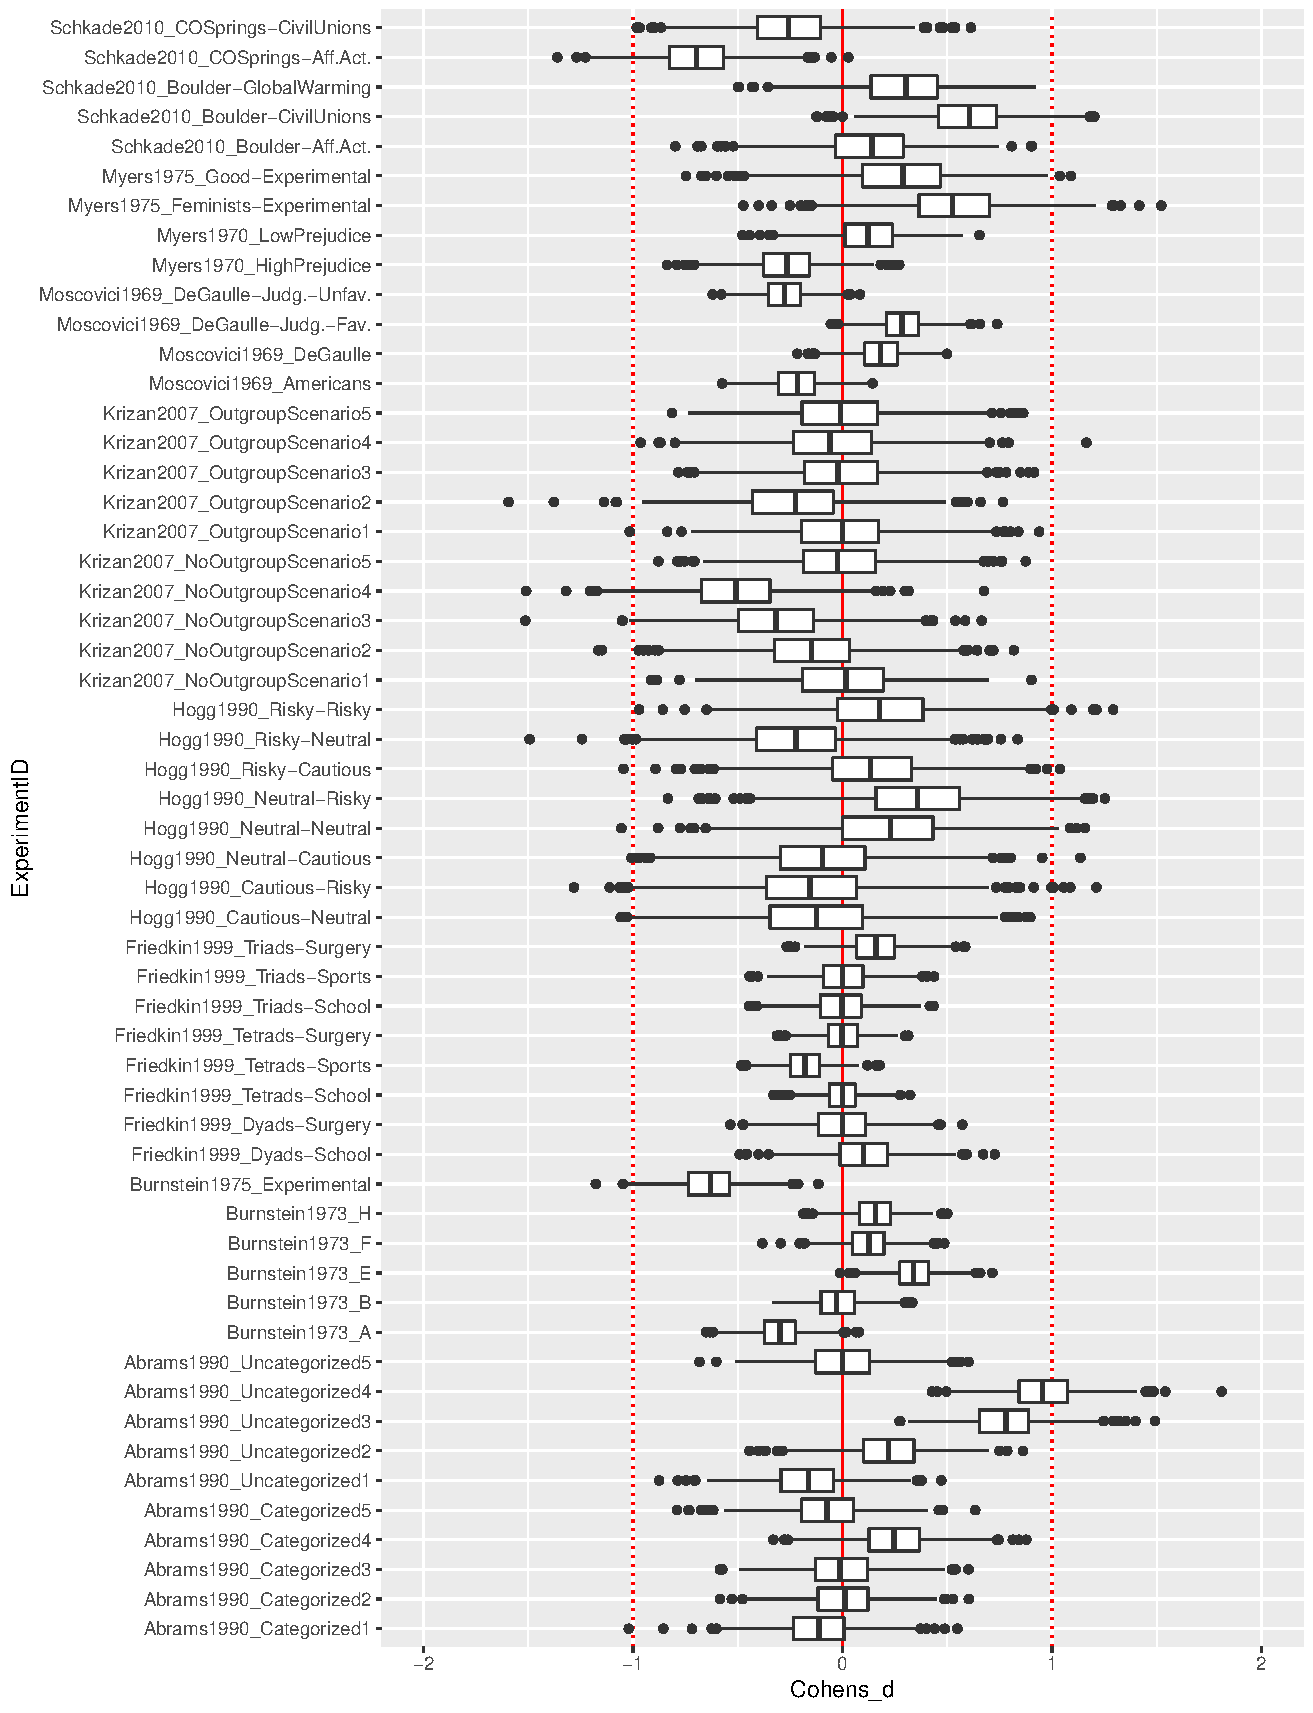
\includegraphics[width=\textwidth]{Figures/boxplots/metric_cohens.pdf}
    \label{fig:MetricBoxplot_N}
  \end{subfigure} \\
\end{figure}
\begin{figure}\ContinuedFloat
  \begin{subfigure}[]{0.9\textwidth}
    % \hspace{-5.5em} 
    \centering
    \textsf{\large \textbf{B}, 10 $\times$ empirical $N$} \\
    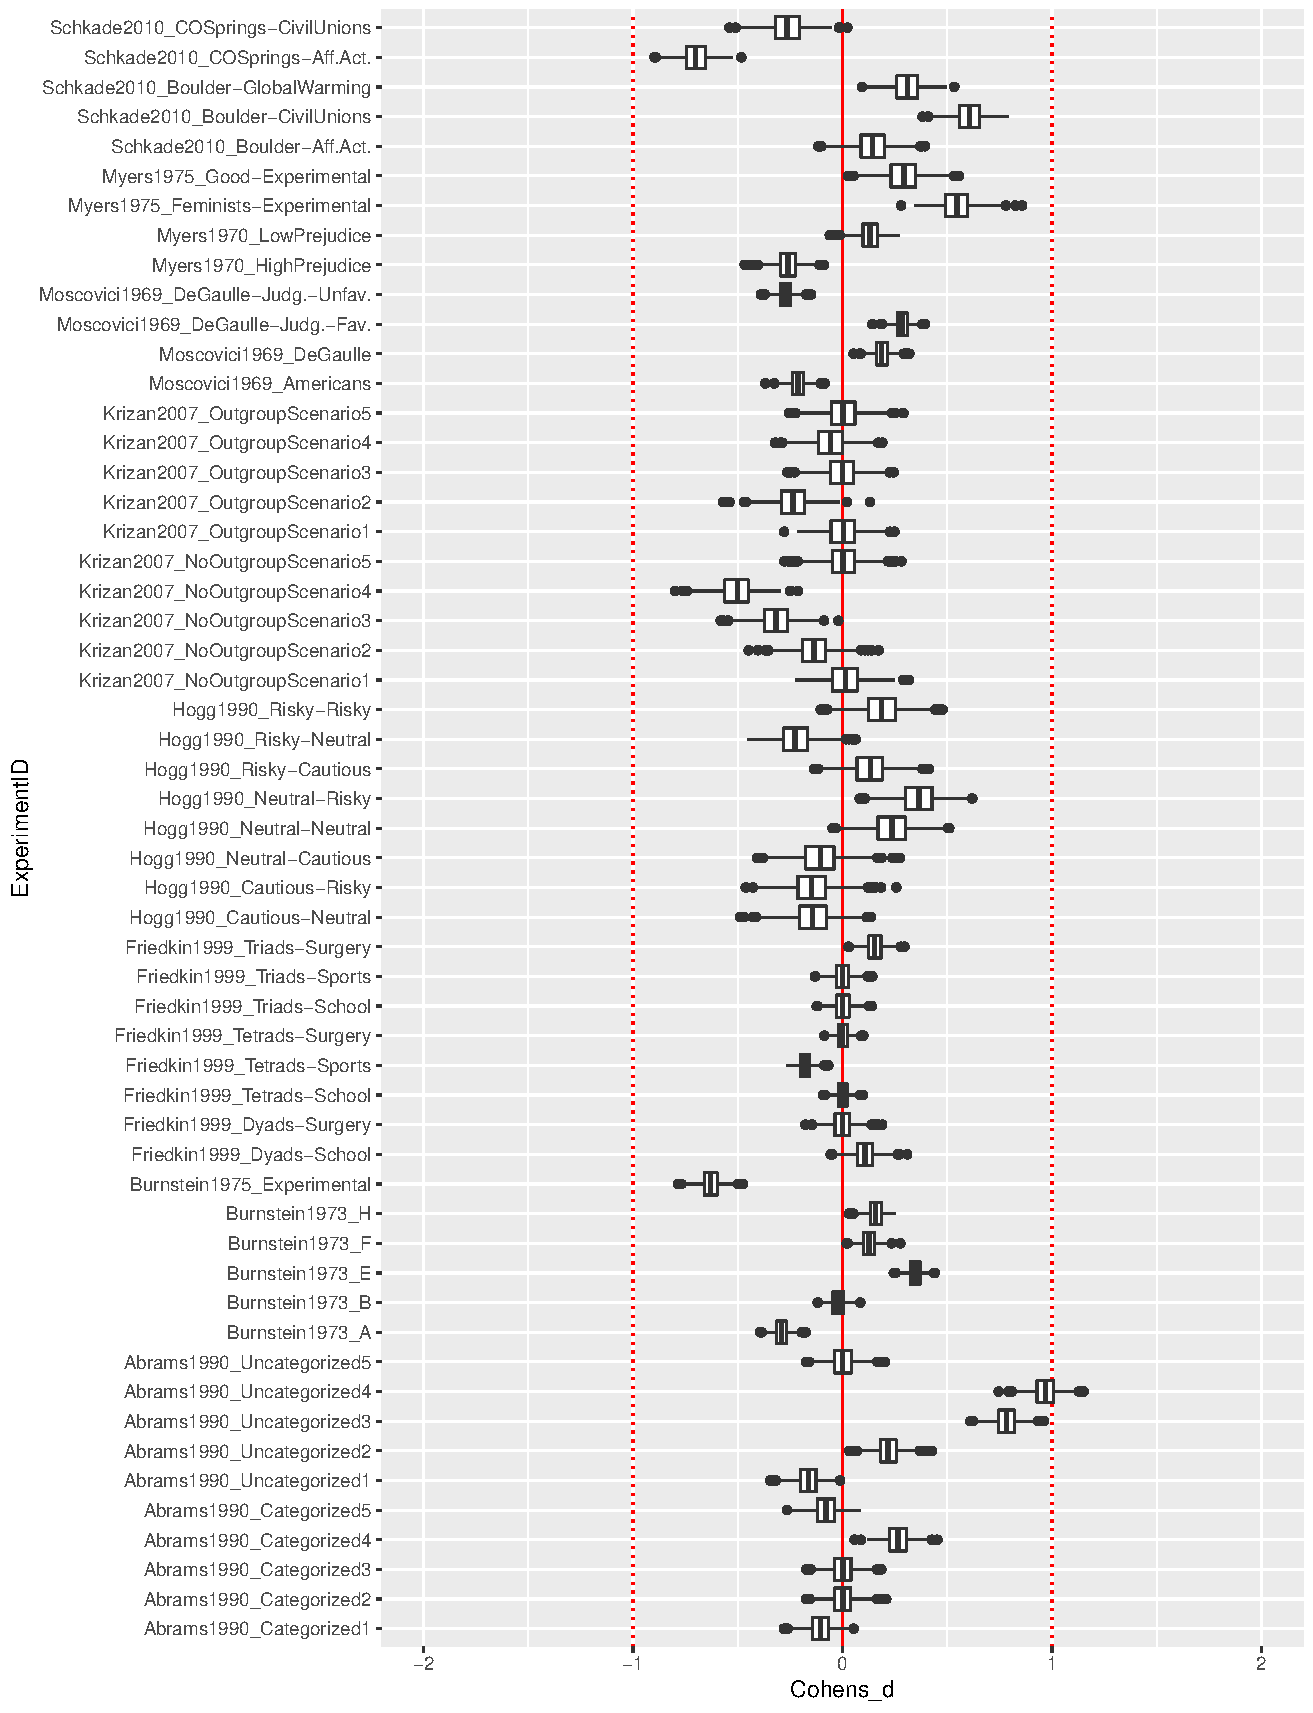
\includegraphics[width=\textwidth]{Figures/boxplots/10N_metric_cohens.pdf}
    \label{fig:MetricBoxplot_10N}
  \end{subfigure}
\end{figure}


\begin{figure}
  \caption{Boxplot of Cohen's $d$ for the ordered probit model over 100
    simulation trias for each experimental condition (y-axis in A and B). Each
    trial represents a possible outcome of a group polarization experiment where
    the true opinion shift is zero. The mean across trials is closer to 0 than
    in the metric case, but many simulated zero-shift experiments still result in
    an observed shift. This illustrates the weak statistical power of these group
    polarization experiments.}
  \label{fig:OrdinalBoxplot}
  \centering
    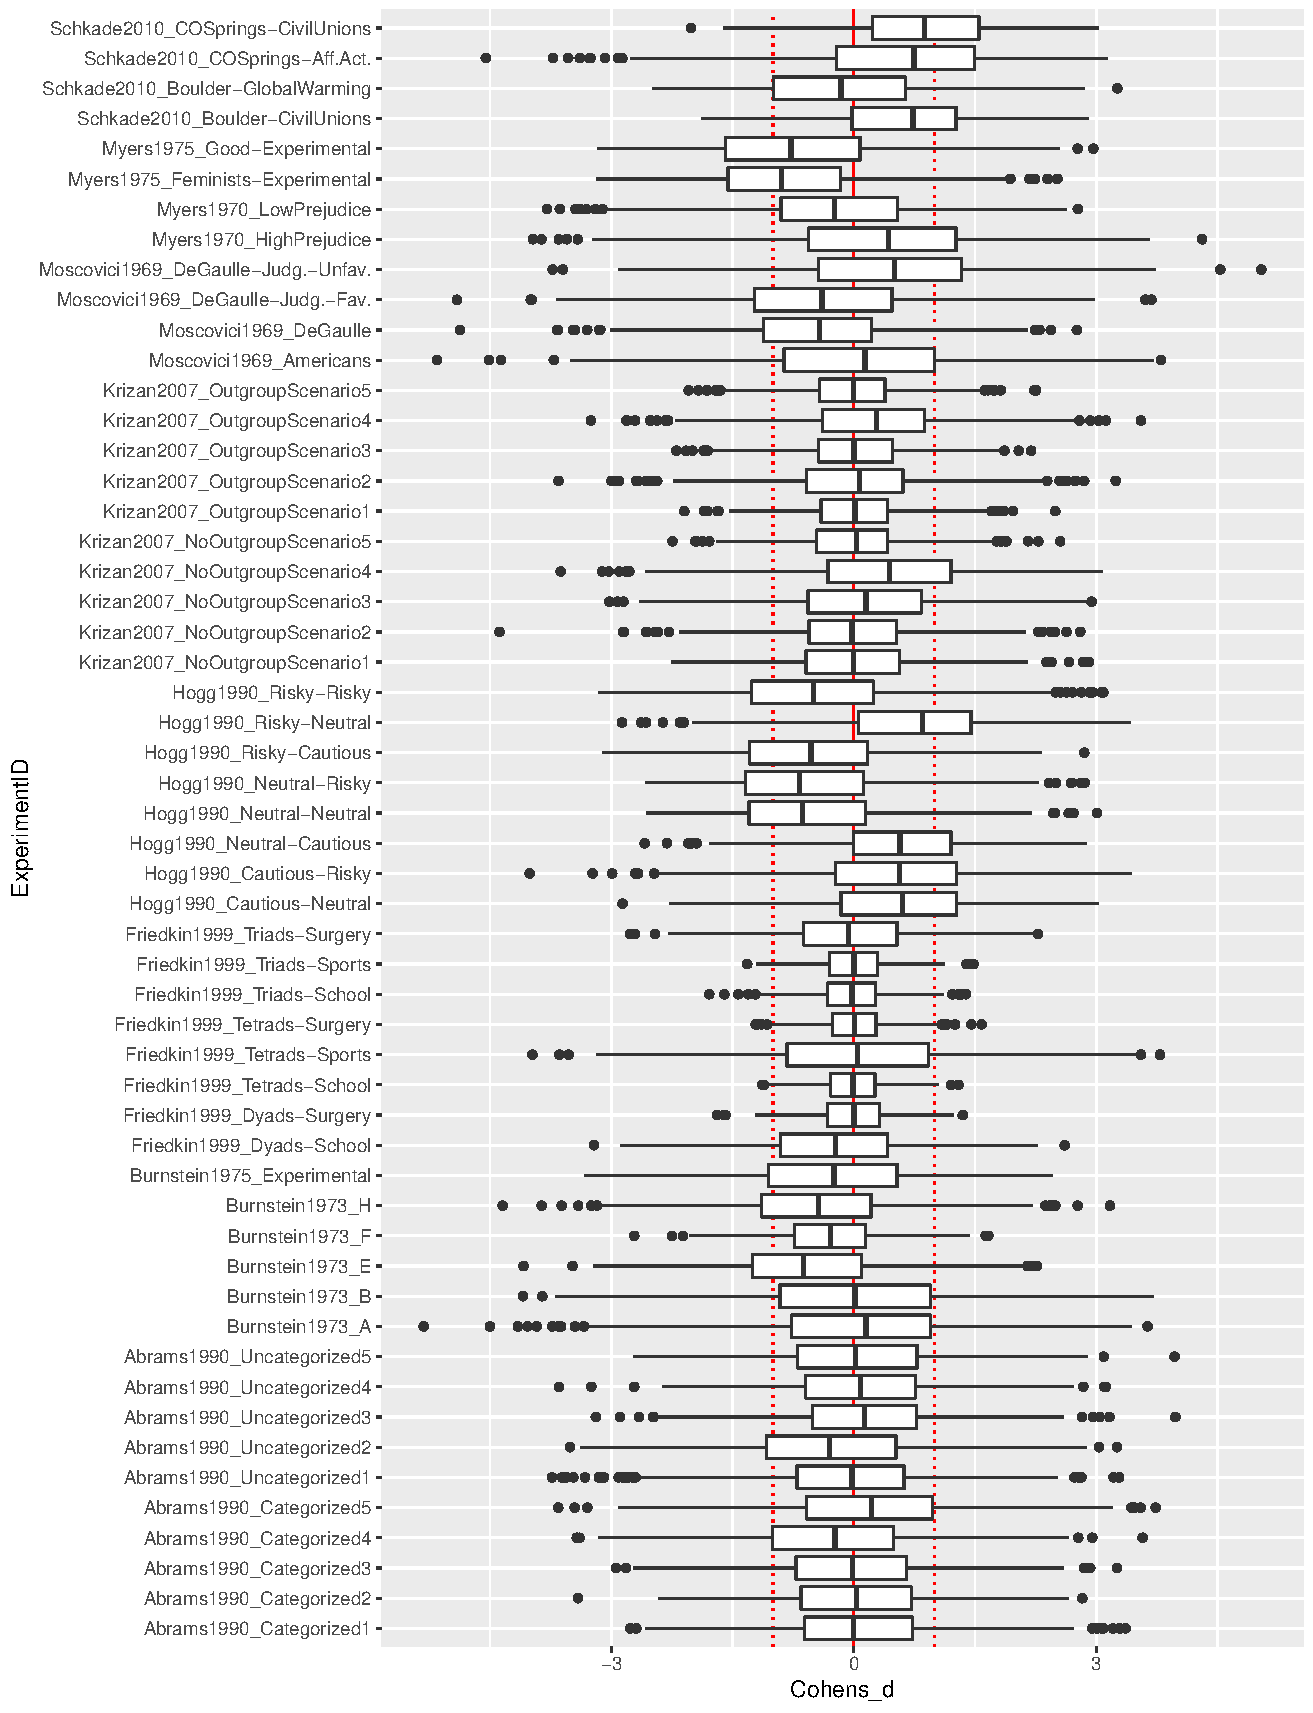
\includegraphics[width=0.9\textwidth]{Figures/boxplots/ordinal_cohens.pdf}
\end{figure}


\end{document}
